\documentclass[sigconf, anonymous]{acmart}

\usepackage{xspace}
\usepackage{listings}
\usepackage{siunitx}

\newcommand{\todo}[1]{{\color{red}{\textbf{\em [TODO: #1]}}}\xspace}
\newcommand{\TODO}[1]{\todo{#1}}




\newcommand{\FigHighLevel}{

\begin{figure}[ht]
    \centering
    % 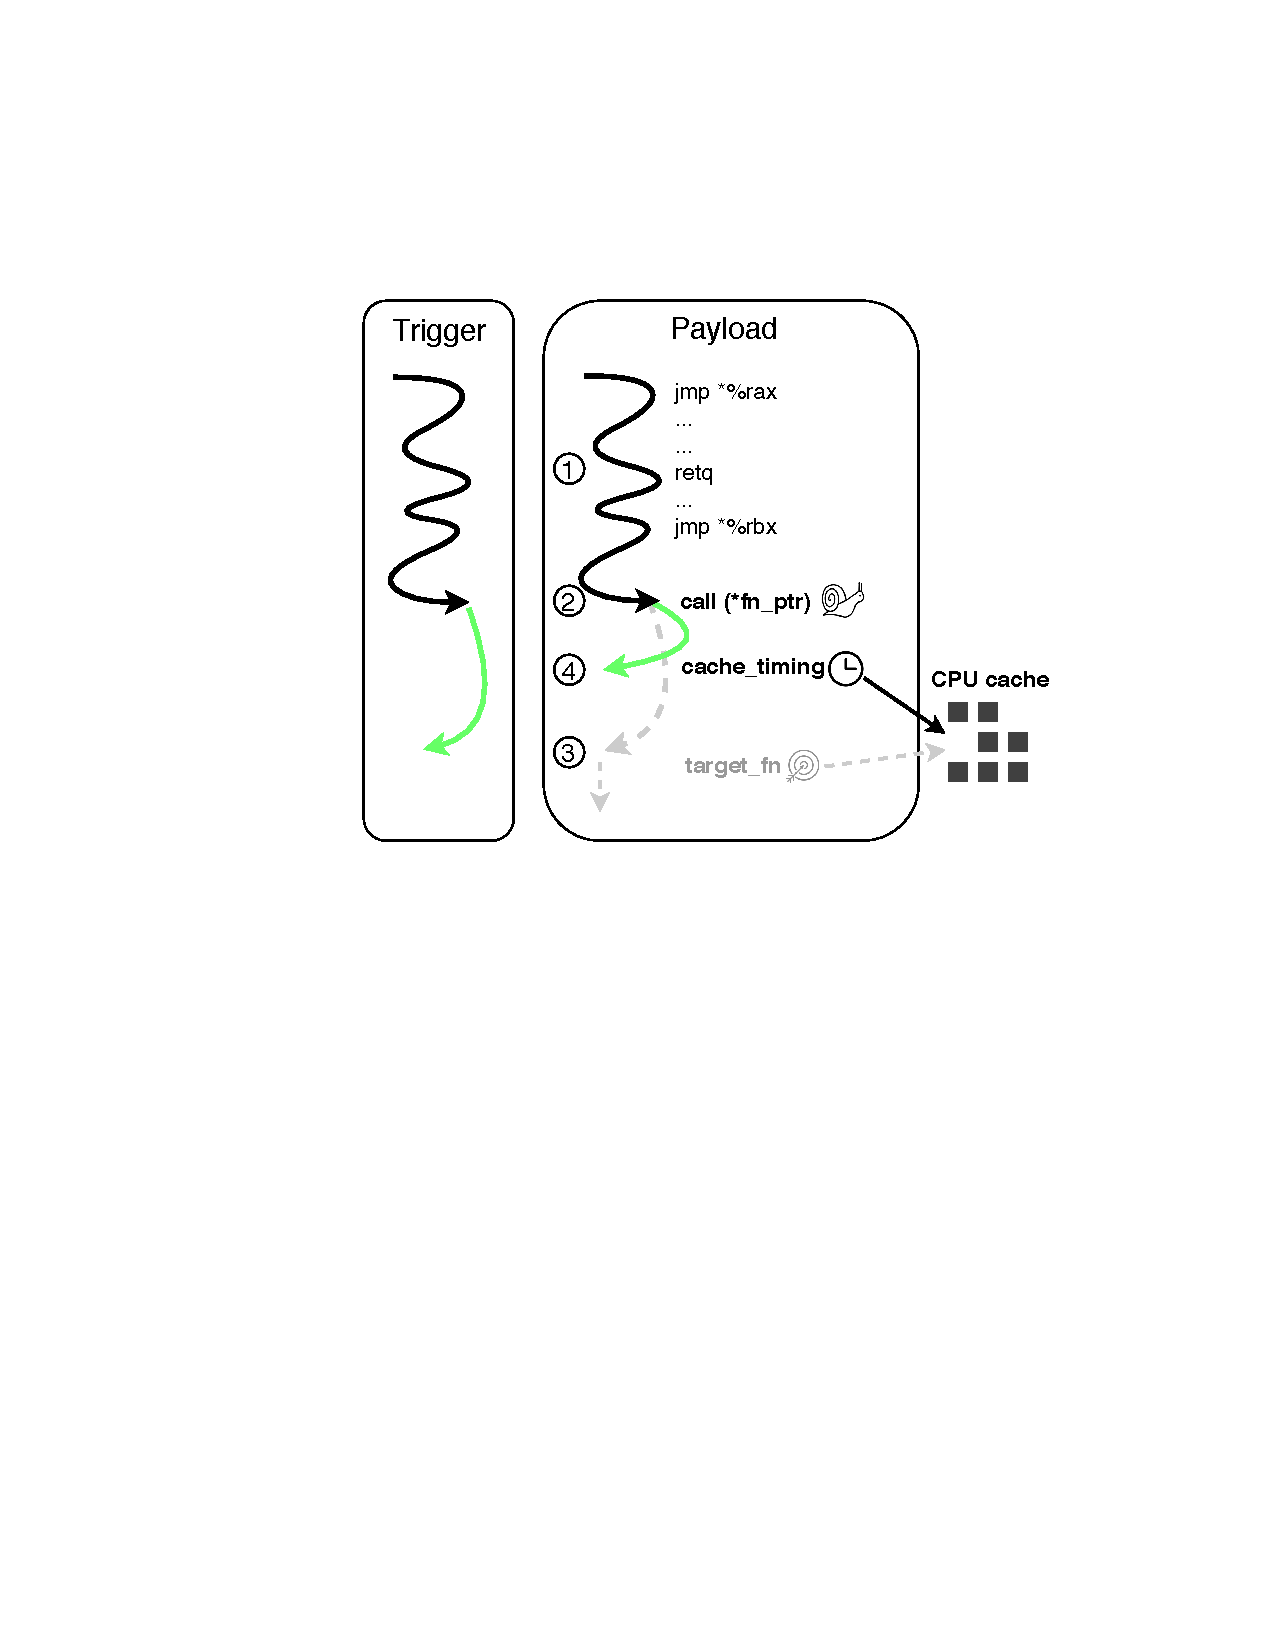
\includegraphics[clip, trim=6cm 13.5cm 3.8cm 5cm, width=0.9\linewidth]{figures/exspectre-high-level.pdf}
    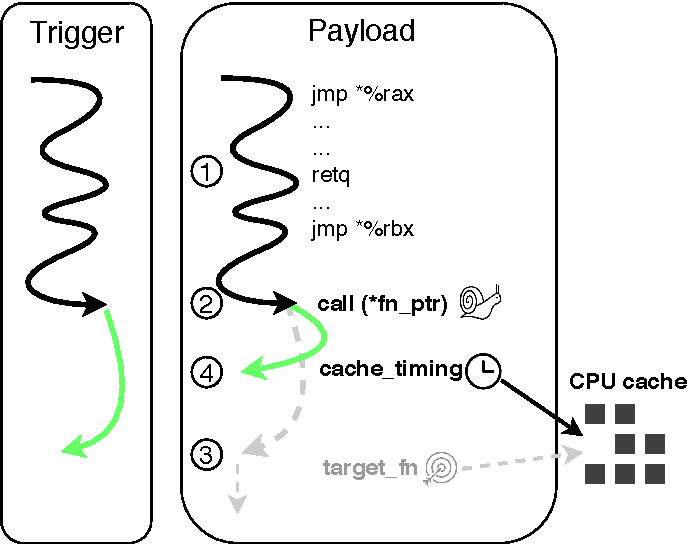
\includegraphics[width=0.9\linewidth]{figures/exspectre-high-level-trimmed.pdf}
    \caption{\textbf{Exspectre}\,---\, %
    1, 2, 3, 4...}

    \label{fig:high-level}

\end{figure}
}


\newcommand{\FigSpecMeasure}{
\begin{figure*}[t]
    \centering
        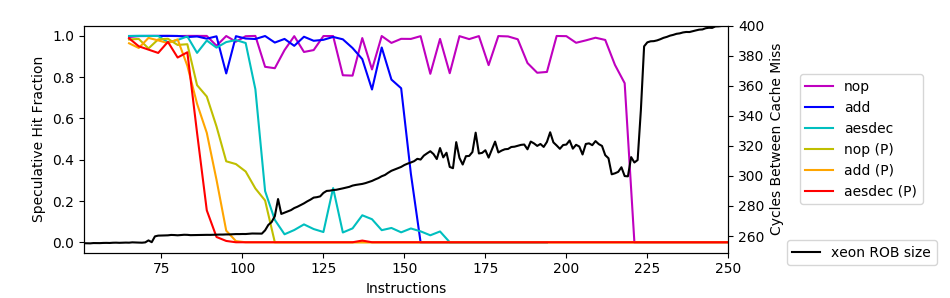
\includegraphics[width=0.9\textwidth]{figures/Speculative_measurements.png}
    \caption{The speculative primitive allows for a limited number of instructions
        to be completed speculatively, dependent on multiple factors. Trigger and 
        payload processes must share cpu resources as they must be performed on 
        the same hyperthread or associated parity hyperthreads. Processes on
        the parity hyperthreads (warm colors) denoted by (P) accomplish a 
        significantly lower number of instructions as compared with processes 
        on the same hyperthread (cool colors).}
    \label{fig:spec-capacity}
\end{figure*}
}


\newcommand{\FigCacheMiss}{
\begin{figure}[t]
    \centering
    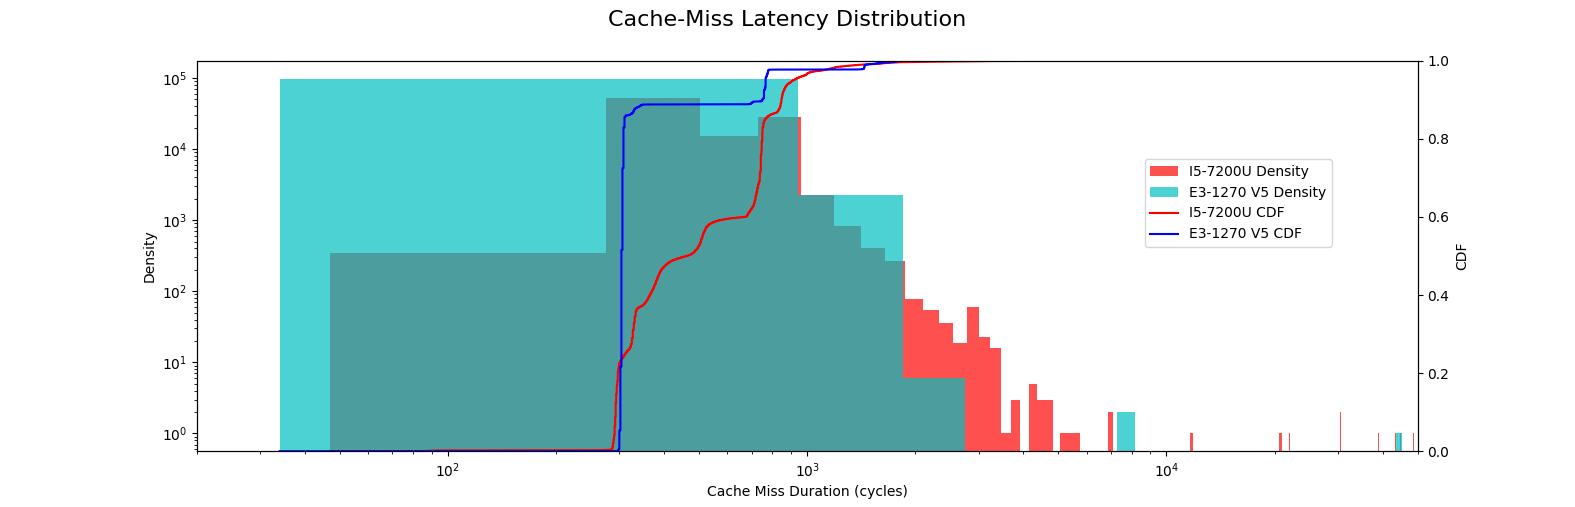
\includegraphics[width=0.5\textwidth]{figures/cache_miss_dist}
    \caption{Cache Hit/Miss Latency Distribution}
    \label{fig:cache-miss}
\end{figure}
}


\newcommand{\FigGeneralModel}{
\begin{figure}[t]
    \centering
        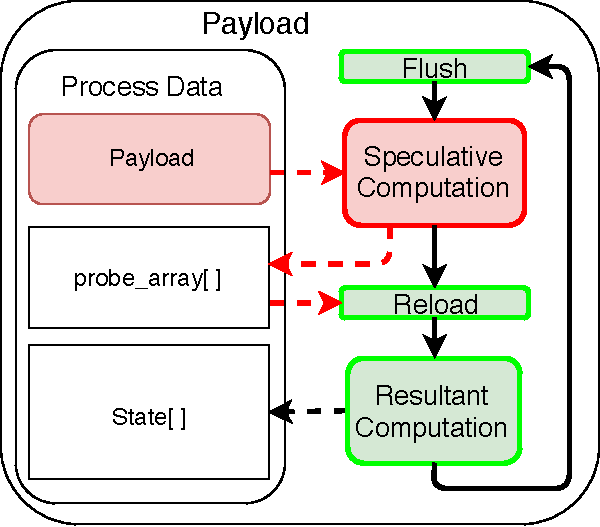
\includegraphics[width=0.4\textwidth]{figures/general_model.pdf}
    \caption{ General model of speculative computation within the Measure 
        process when triggered. \textit{Speculative Computation} has access
        to all variables which do not require a memory transaction within
        the current state of the process. The process can subsequently make
        \textit{Resultant Computations} based on the value returned from 
        \texttt{Flush+Reload} to update the state of the process. }
    \label{fig:general_model}
\end{figure}
}


\newcommand{\FigSpecBandwidth}{
\begin{figure}[t]
    \centering
        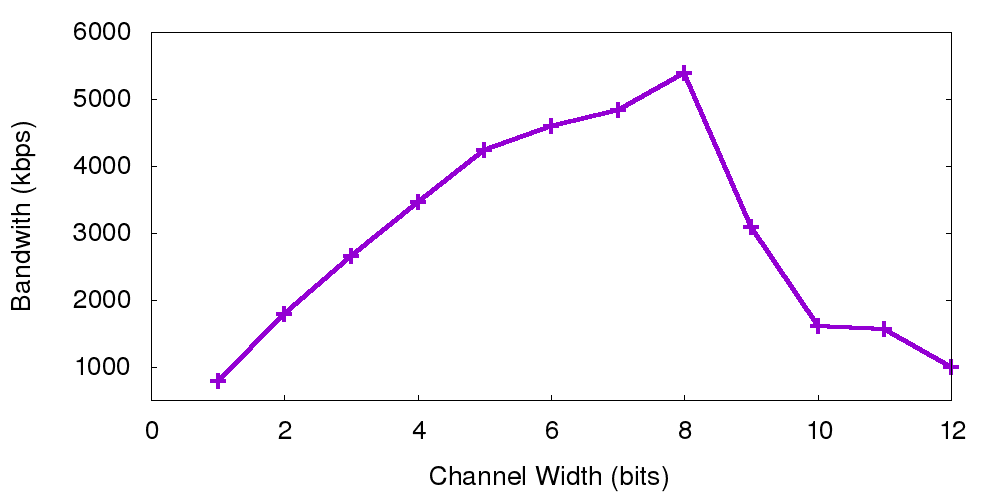
\includegraphics[width=0.5\textwidth]{figures/Speculative_bandwidth}
    \caption{Speculative Bandwidth - Using the speculative primitive 
        1KB of data can be decrypted and exfiltrated at a speed between 5 and 6 kbps
        from the speculative world. Varying the width of the channel 
        results in competing performance factors -- decreasing the 
        number of loops vs decreased size of the probe space.}
    \label{fig:spec_bandwidth}
\end{figure}
}



\newcommand{\FigSpasmModel}{
\begin{figure}[b]
    \centering
        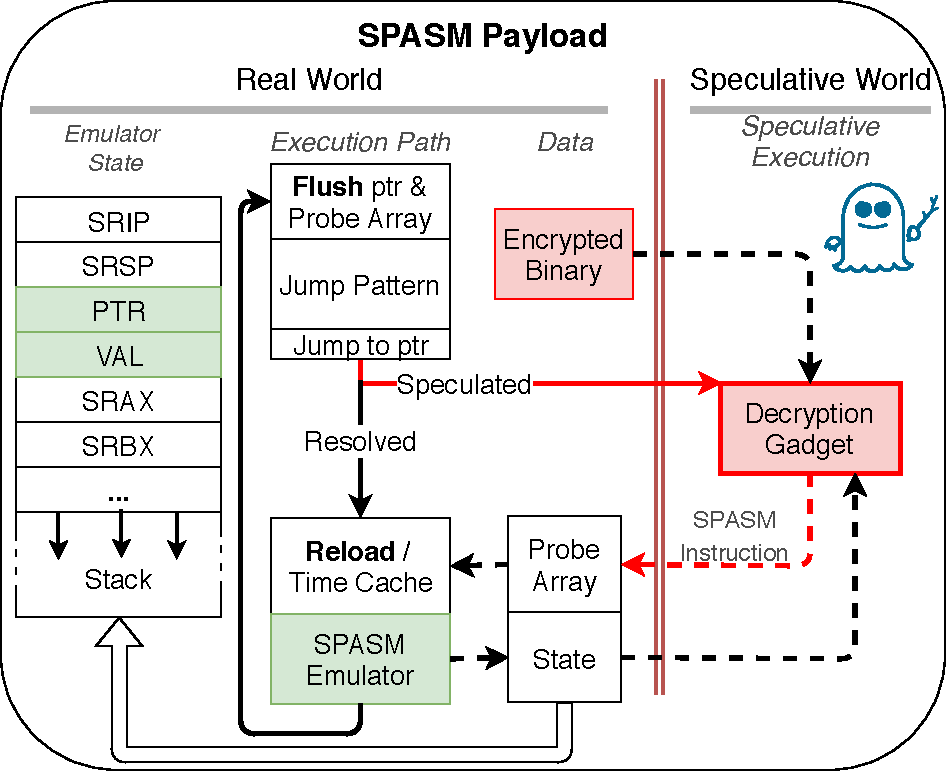
\includegraphics[width=0.5\textwidth]{figures/spasm_model.pdf}
    \caption{This model describes the VM control flow. An encrypted SPASM binary 
        stored in dead code or data accessible to \textit{Speculative Computation} 
        is decrypted  and then returned through the primitive. The SPASM 
        \textit{Resultant Computation} performs the SPASM emulation to update the 
        process state before the next instruction is decrypted.}
    \label{fig:spasm_model}
\end{figure}
}


\fancyhf{} % Remove fancy page headers 
\fancyhead[C]{Paper \#XXX} % TODO: replace 9999 with your paper number
\fancyfoot[C]{\thepage}

\setcopyright{none} % No copyright notice required for submissions
%\acmConference[Anonymous Submission to ACM CCS 2018]{ACM Conference on Computer and Communications Security}{Due 08 May 2018}{Toronto, Canada}
\acmYear{2018}

\settopmatter{printacmref=false, printccs=true, printfolios=true} % We want page numbers on submissions

%%\ccsPaper{9999} % TODO: replace with your paper number once obtained

\newcommand{\speculake}{ExSpectre\xspace}


\begin{document}
\title{\speculake: Hiding Malware in Speculative Execution} % TODO: replace with your title

\begin{abstract}
Recently, the Spectre and Meltdown attacks have revealed serious vulnerabilities in modern CPU
designs, allowing an attacker to exfiltrate data from sensitive programs. These
vulnerabilities take advantage of speculative execution to coerce a processor to
perform computation that would otherwise not occur, leaking the resulting
information via side channels to an attacker.

In this paper, we extend these ideas in a different direction, and leverage speculative
execution in order to \emph{hide malware} from both static and dynamic analysis. Using this
technique, critical portions of a malicious program's computation can be shielded from view,
such that even a debugger following an instruction-level trace of the
program cannot tell how its results were computed.

We introduce \emph{\speculake}, which compiles arbitrary malicious code into a
seemingly-benign payload binary. When a separate trigger program performs a specific
pattern of indirect jumps, it (mis)trains the CPU's branch predictor. Subsequent
executions of the payload binary with similar jumps causes the CPU to mispredict its
branches and speculatively execute a malicious payload, which communicates
results back to the real world via side channels.

We study the extent and types of execution that can be performed in the
``speculative world'', and build tools that enable several computations to be
performed covertly. In particular, within speculative execution we are able to
decrypt memory using AES-NI instructions, and are able to interpret a custom
virtual machine language to perform arbitrary computation.
We also show how the trigger program
can be a pre-existing benign application already running on the system, and
demonstrate this concept with OpenSSL driven remotely by the attacker as our
trigger program.

Finally, we describe defenses, but in all honesty, you're probably not going to like
them.

We consider this to be a new thrust in attack vector research that harkens to work 
done on hardware red-pills and weird machines. We demonstrate that unintended 
functionality of architechture design can be used to compose malicious programs with 
new and different properties. This technique poses novel and unique challenges for 
malware modeling efforts, as it forces an environment to either
faithfully reproduce all hardware behaviors, or overcome a much larger burden of 
reverse engineering. 


\end{abstract}

% TODO: replace this section with code generated by the tool at https://dl.acm.org/ccs.cfm

%\begin{CCSXML}
%<ccs2012>
%<concept>
%<concept_id>10002978.10003029.10011703</concept_id>
%<concept_desc>Security and privacy~Usability in security and privacy</concept_desc>
%<concept_significance>500</concept_significance>
%</concept>
%</ccs2012>
%\end{CCSXML}

%\ccsdesc{Security and privacy~Use https://dl.acm.org/ccs.cfm to generate actual concepts section for your paper}
% -- end of section to replace with generated code

\keywords{Malware; Covert Channel; Weird Machines; TK} % TODO: replace with your keywords

\maketitle


\section{Introduction}


Modern CPU designs use speculative execution to maintain high instruction
throughput, with the goal of improving performance. In speculative execution,
CPUs execute likely future instructions while they wait for other slower
instructions to complete. When the CPU's guess of future instructions is correct, the
benefit is faster execution performance. When its guess is wrong, the CPU
simply discards the speculated results and continues executing along the true path.


Previously, it was assumed that speculative execution results
remain invisible if discarded, as careful CPU design maintains strict separation
between speculative results and updates to architectual state.
However, recent research has revealed side channels that violate this
separation, and researchers have demonstrated ways to exfiltrate results from speculative
computation. Most notably, the Spectre vulnerability allows attackers to leak
information from purposefully mis-speculated branches in a victim
process~\cite{spectre}. The Meltdown vulnerability uses speculative results of an
unauthorized memory read to sidestep page faults and leak protected memory from
the kernel~\cite{meltdown}. Both of these vulnerabilities focus on extracting
secret data from a process or operating system.

\medskip

In this paper, we explore another attack enabled by speculative execution:
\speculake, which \emph{hides computation} within
the ``speculative world''. Taking advantage of the CPU's speculation to secretly
perform computation,
we can produce binaries that thwart existing reverse engineering
techniques. Because the speculative parts of a program never ``truly'' execute,
we can hide program functionality in the unreachable dead code in a program.
Even a full instruction trace, captured by a hardware debugger or software
emulator, will be unable to capture the logic performed speculatively.
This technique could lead to sophisticated malware that hides its behavior
from both static and dynamic analysis.


Existing malware use several techniques to evade detection and
make it difficult for analysts to determine payload behavior of reported malware. 
For example, binary \emph{packers} or \emph{crypters} encode an executable payload as
data that must be ``unpacked'' at runtime, making it difficult to tell
statically what a program will do~\cite{malware-packers}. Malware may also use
\emph{triggers} that only run the payload when certain conditions are present, preventing
it from executing when it is inside an analysis sandbox or 
debugger~\cite{balzarotti2010efficient,red-pill}.

However, with some effort, these existing malware techniques can be defeated.
Analysts can use
dynamic execution to unpack malware and reveal its
behavior~\cite{balzarotti2010efficient}, and can use symbolic execution or code
coverage fuzzers to determine the inputs or triggers that will reveal malicious
behavior~\cite{moser2007exploring,schwartz2010all,wang2017angr,egele2012survey}.


\speculake provides a new technique to malware authors, allowing them to hide
program functionality in code that does not execute at runtime.


At a high level, \speculake consists of two parts: a payload program, and a
trigger program. When run by itself, the payload program executes a pattern of
indirect jumps and measures a cache side channel. While the trigger program is
not running, the payload program is effectively inactive (and may optionally do
some decoy operation). When the trigger program runs, it executes a similar
pattern of indirect jumps (with similar source and destination addresses as the
payload program), effectively training the CPU's branch predictor to the jump
pattern specified by the trigger program.

Importantly, the trigger program and payload program's indirect jump patterns
diverge on the destination of their final jumps. However, because the trigger
program has trained the CPU's branch predictor, the CPU speculates that the
payload program will continue following the pattern of the trigger program,
causing it to execute a \emph{speculative gadget} in the payload
program. This execution path is shown in Figure~\ref{fig:high-level}.

We emphasize that this gadget is in a region that is neither
read nor executed by the payload program, and after the CPU discovers the
mis-speculation in the payload program, it will discard the results from the
speculative gadget and continue executing from the correct destination. However,
the payload program has a limited speculative window where it can perform
computation, and can communicate results back to the ``real world'' payload 
program via a cache side channel.

%Figure~\ref{fig:high-level}


\FigHighLevel



While it's possible for the trigger and payload programs to be bundled in a
single program, an analyst aware of \speculake could easily find the speculative
gadget in the payload program based on the jump pattern in the trigger program.
However, if the trigger and payload are kept separate, the analyst has a much
harder job and must identify both.
Moreover, it is possible that the trigger program be a
seemingly-unrelated benign program already on the victim's computer. We
investigate using the OpenSSL library as a benign trigger
program in Section~\ref{subsec:openssl}. If the trigger program is another benign
program on the system, the analyst has the difficult task of identifying which
program, library, or even operating system component is responsible for training
the CPU's branch predictor, and finding the specific set of jumps that occur at
runtime. To make matters worse, the payload program can include dummy jump
patterns that are effectively dead ends for the analyst, as they do not
ultimately call the hidden speculative gadget.


Simulating or modelling the speculative execution path is a difficult task for a
program analyst hoping to reverse engineer an \speculake binary. First, the
analyst must reverse engineer and accurately model the closed-source proprietary
components of the target CPU, including the branch predictor, cache hierarchy,
out-of-order execution, and hyperthreading. In contrast, the \speculake
author only has to use a partial model of these components and produce binaries
that take advantage of them, while the analyst's model must be complete to
capture all potential \speculake uses. Second, the analyst must run all
potential trigger programs through the simulator, including benign programs with
realistic inputs. Both of these contribute to a time-consuming and expensive
endeavor for would-be analysts.

% Results summary
In order to study the potential of \speculake, we implement several example
payload programs and evaluate their performance. We find that the speculative
window is limited by the reorder buffer and physical register file sizes, which
allows us to execute between 100 and 200 instructions speculatively on modern
Intel CPUs. While brief, we are able to perform execution in short steps,
communicating intermediate results back to the ``real world'' part of the
payload program. Using this technique, we demonstrate implementing a universal
Turing machine (demonstrating arbitrary computation), a custom instruction set
architecture that fits within the constraints of speculative execution, and show
the ability to perform AES decryption of a text block via AES encrypt/decrypt
instructions.

Using these building blocks, we demonstrate the practicality of hiding arbitrary
computation by implementing a reverse shell in our speculative instruction set.
We show that this simple payload is able to perform several system calls
in a reasonable time, ultimately launching a dial-back TCP shell in under 7~seconds after
the trigger program starts.

%Using these building blocks, we demonstrate the practicality of hiding arbitrary
%computation by decrypting an AES-encrypted ARM binary in the speculative world
%one instruction at a time, returning the decrypted next instruction to the real
%world part of the payload program, which updates a virtual machine. We show that
%we are able to decrypt and process approximately 25 instructions per second.


% contributions?
% - explore the limits of speculative execution
% - propose novel concept of hiding computation in speculative execution
% - implement example applications using this concept, including decrypting
%   data speculatively
% - demonstrate using benign program (openssl) as trigger
% - identify defenses and discuss ways to counter them



% Move to discussion:
% TODO: we don't talk at all about how an analyst might try to enumerate
% the potential entry points to the speculative world, and how that can be
% made difficult




%%%%%%%%%%%%%%



\section{Background}
Modern CPU designs employ a wide range of tricks in order to maximize
performance. In this section, we provide preliminary background as they are
relevant to our system, as well as a brief summary of the Spectre vulnerability.

\subsection{Out-of-Order Execution}
Many CPUs attempt to keep the pipeline full by executing instructions \emph{out of
order}, with the CPU allowing future instructions to be worked on and executed
while it waits for slower or stalled instructions to complete. To maintain
correctness and the original (Von Neumann) ordering, instructions are tracked in
a \emph{reorder buffer} (ROB), which keeps the order of instructions as they are
worked on out of order. Instructions are \emph{retired} from the ROB when
they are completed and there are no previous instructions that have yet to
retire. Upon retiring, an instruction's results are committed to the architectural
state of the CPU. Thus, the ROB ensures that the program (or debugger) view
of the CPU state always updates in program execution order, despite out of order
execution.

\subsection{Speculative Execution}

CPUs also attempt to keep their pipeline full by predicting the path of
execution. For example, a program may contain a branch that depends on a result
from a prior slow instruction. Rather than wait for the result, the CPU can
\emph{speculatively execute} instructions down one of the paths of a branch,
storing the results of the speculative instructions in the ROB.
If the guess of the branch target turns out to be correct, the CPU can quickly
retire all the instructions it has speculatively executed while waiting. If the
guess is incorrect, the CPU must discard the
(incorrectly) speculated instructions from the ROB, and continue executing from the
correct branch target.


\subsection{Branch Prediction}
When a CPU mispredicts a branch, the speculative execution results are
discarded, costing the CPU several cycles as the pipeline is flushed. To
minimize this, CPUs employ \emph{branch predictors} that attempt to guess the
path of execution. Branch predictors maintain a short history of previous
branch targets for a particular branch (e.g. whether a certain branch is
frequently taken or not taken), and use
this to inform the CPU's guess for speculative execution.

There are two kinds of branches a CPU handles: \emph{direct} and
\emph{indirect}. A \emph{direct} branch may either jump to a provided address or
continue executing straight through depending on the state of the CPU (e.g. condition
registers). While there are only two potential statically-known targets for a direct
branch, the CPU may not know if the branch is taken or not until preceding
instructions retire. An \emph{indirect} branch is always taken, but its address
is determined by the value of a register or memory address. Direct branches are
typically used for control flow such as \texttt{if} or
\texttt{for}/\texttt{while} statements, while indirect branches are used for
function pointers, class methods, or case statements.


%- BHB, BTB

\subsection{Spectre}

In early 2018, researchers revealed the Spectre vulnerability, which allows an
attacker to leak information from a victim program~\cite{specte}. Spectre uses
the fact that speculative execution can influence system state via side
channel. In Spectre, an attacker mistrains the branch predictor of a CPU running
a victim program by providing inputs to it. Once mistrained, the attacker then
sends a new input that will cause a different in-order execution path. However,
because the CPU's branch predictor has been mistrained, it will still
speculatively execute the previous path.

Consider the following code snippet from the Spectre
paper~\cite{spectre}:

\begin{lstlisting}
    if (x < array1_size)
        y = array2[array1[x] * 256];
\end{lstlisting}

The \texttt{if} statement correctly protects an out-of-bounds reads from \texttt{array1}.
But if the branch predictor makes an incorrect guess on the branch's direction
and speculatively executes inside the \texttt{if} statement, it may
cause a read beyond the boundary of \texttt{array1}. The result of this will
then (speculatively) be multiplied by 256 and used as an index into
\texttt{array2}. Although the CPU will not commit
the speculative update to \texttt{y}, it will still issue a memory read to
\texttt{array2[array1[x]*256]}, which will be cached. Importantly, even after
the CPU realizes the branch misprediction, it does not rollback the
state of the cache, as this does not directly influence program correctness.
However, the set of cached values is observable to the program via a
side-channel: by timing reads to \texttt{array2[i]}, the fastest read will
reveal the speculative value of \texttt{array1[x]*256}, for any value of
\texttt{x}. An attacker that is able to perform such a side-channel inference on
the cache can learn the speculative result of an out-of-bounds read from
\texttt{array1}.


Spectre can also be applied to indirect branches. Branch predictors use the
history of previous branches to predict the destination of an indirect jump when
the destination is not yet known. For direct branches, only one of two
destinations (taken or not taken) are possible to speculatively execute. But for
indirect branches, a mistrained branch predictor can potentially be coerced into
speculatively executing from \emph{any} target instruction in the binary.

We take advantage of the behavior of indirect branch prediction to hide the
location of our speculative computation.
%TODO more on why this is crucial...

%%%%%%%%%%%%%%




\section{Architecture}
\speculake malware is comprised of two independent pieces: a payload program,
and a trigger. The payload, and some form of the trigger, must be installed
on the victim's computer (e.g. via trojan, remote exploit, or phishing). A running
payload performs innocuous operations while waiting for the trigger to
become present.

One form the trigger can take is another local program that interacts with the
payload via the indirect branch predictor. In this case, both programs must run
on the same physical CPU. We note that this constraint is not a significant
burden, as programs can either use \texttt{taskset}, or, if not available, run
multiple instances or wait for the OS scheduler to execute both programs on
the same core.

At a high level, the trigger program performs a series of indirect jumps in a
loop, training the branch predictor to this pattern. Meanwhile, the
payload program performs a subset of this jump pattern, then forces the CPU to
speculate by stalling the resolution of an indirect branch via a slow memory
read. The CPU will (mistakenly) predict the jump to follow the pattern performed
by the trigger program, and speculatively execute that destination in the
payload program.

The trigger can also take the form of a special input to the payload program,
rather than a separate program.
In this case, the payload program parses input data and performs innocuous
operations with it. Once the trigger input is provided, it causes the program to
\emph{speculatively} overflow a buffer, despite correct bounds checks in the program.
The speculative buffer overflow (described in
Section~\ref{subsec:spec-buffer-overflow}) causes the program to speculatively
execute at an address chosen by the trigger input and controlled by the
attacker.


\subsection{Threat Model}

We assume a scenario where an adversary wishes to hide or obscure the behavior
of a malicious program (malware) from an analyst attempting to reverse engineer
it. We note this is distinct from the goals of evading malware detection, where
malware escapes classification by an anti-virus or other automated tool. While
we believe \speculake could also be used to make automated detection more
difficult, our main focus is on reverse engineer resistance, useful for evading
manual classification concerned with malware behavior. For anti-virus evasion,
we refer the reader to several existing techniques that are sufficient to defeat
existing anti-virus
systems~\cite{jana2012abusing,oberheide2009polypack,ropinjector,swinnen2014one,ugarte2015sok}.


We assume the adversary is able to install binaries on the target machine (e.g.
via a trojan or remote exploitation), and the analyst is attempting to determine
what the malware will do using traditional debugging tools. We assume the
analyst may be aware that speculative execution is used to obfuscate behavior,
but does not have special-purpose hardware that allows introspection of the
CPU's speculative state. This assumption is realistic, as modern processors do
not allow developers or other users to directly interact with proprietary CPU
optimizations and features.

We further assume that the malware has a specific trigger that the analyst is
not privy to, and the adversary can influence. In our examples, this
trigger is often behavior exhibited by some other (potentially benign) process
running on the same system as the malware. As the adversary is able to control
when such a trigger is deployed (potentially remotely), the analyst will not be
able to observe or force this trigger to happen at will. We emphasize that while
this may also be true for existing trigger-based malware, analysts can often
reverse engineer the trigger out of the malware, for example by observing
control flow within the malware and using adaptive
fuzzers~\cite{afl,stephens2016driller} to generate inputs that explore other
execution paths of the binary. In contrast, \speculake malware's trigger
influences behavior of the payload program speculatively, making it effectively
invisible to the analyst. As with typical
malware, the analyst may attempt to reverse engineer the trigger to reveal the
malware's behavior, but we will show (in Section~\ref{subsec:nested-spec}) how
this type of analysis can be defeated.

\subsection{Indirect jumps}


In \speculake, we cause the CPU to mis-speculate the destination of an indirect
branch in the payload program, causing it to speculatively execute 
instructions that are never truly executed. We term the destination where speculation begins
the \emph{speculative entry point}. \speculake uses indirect jumps to allow
speculative execution from \emph{any} instruction in the payload process'
address space. Because it can jump to any instruction, the malware analyst has a
difficult task in determining where a payload program's speculative entry point
is.

In fact, the location of this entry point is not determined by the payload
program, but rather the corresponding trigger program. This means that with only
the payload program, an analyst does not posses enough information to find the
speculative entry point.

In this section, we will describe the trigger program variant, and discuss how
input data can be used a speculative trigger in
Section~\ref{sec:spec-buffer-overflow}.

Indirect branch predictors allow the CPU to predict the destination address of a
branch based solely off its source address and a brief history of previous
branch sources and destinations. While the inner-working details of modern CPU
branch predictors are proprietary, it is possible to reverse engineer parts of
their behavior, which we do for \speculake.

We observe that Intel CPUs consider three types of x86\_64 indirect branches:
\texttt{retq}, \texttt{callq *\%rax}, and \texttt{jmpq *\%rax}\footnote{other
general purpose registers besides \texttt{\%rax} can be used as well}.
We created a simple trigger program that performs a series of 28 indirect
branches
using \texttt{jmpq *\%rax} instructions, as we found that 28 jumps was the minimum
needed to reliably train the indirect branch predictor. 
Between each jump, we incremented
\texttt{\%rax} accordingly to continue on to the next jump. After these 28
jumps, we load a function pointer into \texttt{\%rax} and do a final indirect
branch using \texttt{callq *\%rax}. In our trigger, we perform these jumps
        repeatedly in a loop.

In our payload program, we first perform the same 28 indirect jumps. We ensure
the source and destination addresses of these jumps is the same as in the trigger program by
manually defining their containing function at a fixed address inside a linker
script. We also do the final indirect call to a function pointer, but with two
differences. First, the destination in the function pointer is a different
address, and second, the memory location of the function pointer itself is uncached.
This forces the CPU to predict the destination of the final indirect call while it
waits for the function pointer to load from memory. Due to the similar
history of branches with the trigger program,
the CPU will (incorrectly) predict the destination to be the same as the one in
the trigger program, which determines the speculative entry point for the
payload. Even though the in-order execution of
payload program never executes or even reads from this address, the CPU will
briefly execute instructions there speculatively.

Eventually, the de-reference of the uncached function pointer in the payload
program will be resolved, and the CPU will recognize it has incorrectly
predicted the destination of its \texttt{callq} instruction. The results from
the speculative entry point instructions will be discarded, and the CPU will
continue executing from the correct destination. However, the speculative code
can change what is loaded into the cache based on its computation, allowing it
to covertly communicate its results to the ``real world'' program.



\subsection{Limits of Speculative Execution}

\FigCacheMiss

\FigSpecMeasureNP

We performed several experiments to determine how much computation can be
performed
speculatively, as well as what components are responsible for the limit.
We report results from our experiments on an Intel~Xeon-1270 (Sandy Bridge),
though we note we found similar results across other Intel processor generations,
including an i5-7200U (Kaby Lake), % jack
an i5-4300U (mobile Haswell), % ewust laptop
an i5-4590 (desktop Haswell), % ewust desktop
as well as an AMD EPYC 7251. % envy
% For simplicity, we report results from only the Xeon-1270.



\subsubsection{Cache Miss Duration}
When executing instructions speculatively we rely on a memory load of a function
pointer from uncached memory. Thus, one potential limit on our computation comes
in the form of the time it takes for the memory read to return with a result
(and for the CPU to determine the result was mis-predicted).
We measured the number of cycles a
cache miss takes to return by artificially evicting an item from cache and
timing reads from its address.
Figure~\ref{fig:cache-miss} shows the CDF of cycles taken. In the typical case,
an evicted item takes approximately 300 clock cycles to load from the Level 3 cache (L3), which
would allow a limit of roughly 200 speculative instructions to be
executed during that time. We note that when an item is not in L3, it takes
considerably longer to load, in theory allowing for thousands of speculative
instructions in a significant fraction of runs.


\subsubsection{Reorder Buffer Capacity} \label{sssec:ROB}
We also measured the capacity of the reorder buffer (ROB) using a method
outlined by~\cite{measuring-rob}. We measure the maximum number of cycles taken
to perform two uncached memory reads, and vary the number of filler instructions
between them. If the number of filler instructions is small, both memory reads
will fit inside the ROB, and it can issue their memory reads in parallel.
However, if the filler instructions fill the ROB, the second memory read will
have to wait for the first to return before it can be issued, causing a
noticeable step increase in the cycle count. Figure~\ref{fig:spec-capacity-np}
shows this step occurs at approximately 220 instructions for our processor,
suggesting a hard upper bound regardless of how long the cache miss takes to
resolve.

%TODO: explain why it's noisy? why does the maximum number of cycles drop below
%this when we're above 220 instructions? Is the step somewhere above that, but
%other processes have crept in (but occasionally, we get lucky and it's just us)?

\subsubsection{Speculative Instruction Capacity}

To verify the upper limit of speculative instructions, we instrumented our
trigger and payload programs to test a simple gadget of variable-length before it
communicated a signal to the real world via a cache side channel. If the cache
side channel revealed no signal in the real world, then we know the speculative
execution did not make it to the signal instructions before the mis-speculated
branch was resolved.

We also tested whether instruction complexity or data dependencies impact the
number of instructions that can be completed. We find that data dependencies and
instruction complexity both have an impact on the number of instructions that
can be executed. Instruction complexity is determined by the number of $\mu$~ops
that the instruction uses, which appears to be what is tracked in the ROB. For
instance, on our architecture, the 64-bit \texttt{idiv} instruction takes 59~$\mu$~ops,
and we can execute up to 3 of them in the speculative world.
Meanwhile, we can execute up to 18 32-bit \texttt{idiv} instructions, which each
take 9~$\mu$~ops~\cite{intel-instruction-tables}. These suggest we can execute
on the order of 175~$\mu$~ops before the speculative world expires.

% We found that the processor can identify some operations that have no effect on
% output registers and allows them to use the entire size provided by the ROB, as
% determined in Section~\ref{sssec:ROB}. This includes idiomatic no-ops and zero
% idioms, which have no reliance on register values, for example the instruction
% \texttt{xchg \%rax, \%rax} and \texttt{xor \%rax, \%rax}. However, if an
% instruction is a potential data hazard, it must use an entry in the Physical 
% Register File (PRF) until it reaches the correct stage in the execution pipeline. 
% In this case, the number of instructions could be limited by the PRF
% entries available.
% 
% %TODO: is this true? Or better explained by the micro-op story?

Most notably instructions that use the extended x86 registers are still valid
within the speculative context. Specifically, Intel's hardware accelerated
AES-NI encryption and decryption instructions, which each use 128-bit registers.
As shown in Figure~\ref{fig:spec-capacity-np}, speculative environments can
complete a significant number of AES rounds---over 100 rounds in our
experiments, more than enough to decrypt a
full block using simple AES modes (e.g. AES-CTR). We investigate the use of AES
instructions in the speculative environment further in
Sections~\ref{subsec:decryption}.

\medskip

We find that when executing speculatively, the number of instructions completed
is rarely limited by cache miss duration. Instead
ROB size and processor mechanisms for resolving
data dependencies define an upper boundary of approximately 150
instructions\footnote{While \texttt{nop} is able to execute up to the full 220
ROB capacity, instructions that do useful work (and/or use multiple $\mu$ ops) cannot reach this limit}.

% TODO: 
% - Highlist instruction signal variablity (add v mul v aesdec v nop)?
% - Limitation is in the ROB (cite other work that supports this)
% - MORE PROCESSORS for testing?
% - ARM?


\subsubsection{Hyperthreading}
\label{sssec:hyperthread}

\FigSpecMeasureParity

When running our tests, we assign the payload and trigger program to the same
core using \texttt{taskset}. We note in the absence of \texttt{taskset}, we can
run multiple instances of trigger programs to occupy all cores, eventually
having the payload program and trigger program become co-resident.

We also explore using hyperthreading, where the CPU presents two virtual cores
for each physical core, allowing the OS to schedule programs to each
simultaneously. In effect, this can cause the interleaving of instructions
between two programs to be much finer-grained: at the instruction level rather
than changing only at the OS-controlled context switch. We find that this
has two effects on speculative programs. First, the finer-grained interleaving
allows for a higher hit rate from the cache, suggesting that each indirect jump
pattern is more likely to result in speculatively executing from the intended
position. % TODO: can we quantify this?
Second, because the physical CPU is being shared, it effectively halves the
number of instructions that can be run in the speculative context.
Figure~\ref{fig:spec-capacity-parity} shows the instructions that can be run when
running trigger and payload on a single core vs.\ a pair of hyperthreaded cores.

We note that Single Thread Indirect Branch Predictors (STIBP) have been implemented
in most environments to prevent cross thread branch predictor interference.
While this does remove the \speculake trigger's influence in scenarios where a
process runs on an isolated cpu, in most modern environments
tasks are scheduled to all available processors. This means that the trigger and
payload will be coresident eventually, allowing progress to continue.


\subsubsection{Nested Speculation}
\label{sssec:nested-spec}

We explore the ability for the CPU to ``double speculate'', where a second
stalled indirect jump while the CPU is already speculating causes it to predict
the target and
speculate a second time. For instance, suppose a payload program truly jumps to
target A, but the CPU is mistrained by a trigger program that jumps to B, thus
causing the payload program to speculatively execute at B. At B, suppose there
is a second indirect jump, perhaps using the same register as the first jump
(which has still not resolved). If the trigger program jumps to C, the payload
program may speculate a second time and continue speculative execution at~C.

We find that not all Intel CPUs support nested speculation. For
example, it appears Haswell chips do not speculate while already speculating,
but nonetheless support non-nested \speculake. Both Sandy Bridge (which
preceded Haswell) and Kaby Lake (which followed Haswell) support nested
speculation. We find that when a CPU does support nested speculation, there
appears to be no limit to nested depth besides the speculative instruction
limit. We use a 16-deep nested speculation in Section~\ref{subsec:impl-aes}
to protect speculative decryption keys from reverse
engineering.

\subsection{Speculative Primitive}

We summarize our findings into a \emph{speculative primitive}, which allows our
payload program to speculatively (and covertly) perform on the order of 100
arbitrary instructions while an accompanying trigger program is running, and
communicate a short (e.g. single byte) result to the real world via a cache side
channel. These speculative instructions are able to read from any real-world
memory or registers, but they cannot perform updates or writes directly. To
update memory, the speculative instructions must communicate to the real world.
We use a cache side channel to do so, but other side channels compatible with
Spectre could also be used~\cite{kiriansky2018speculative}.

We note a performance tradeoff between the size of communication (e.g. 4 bits vs
8 bits) and the time it takes the real world to recover the result from the side
channel. Using Flush+Reload~\cite{yarom2014flush+} as our cache side channel,
recovering the result requires accessing all elements in an array exponential in
the size of the result (e.g. $2^8$ array reads to recover an 8-bit result).
Therefore, there is a performance advantage for keeping the size of the result
small, and communicating out small pieces of information that are aggregated by
the real world over multiple speculative executions. Meanwhile, smaller channels
introduce more overhead in recovering information. We investigate this tradeoff
in Section~\ref{subsec:impl-aes}, and find that 8~bits is near optimal in
practice.

%%%%%%%%%%%%%%



\section{Application Payloads}

While the amount of computation done in a single speculative execution is small,
we demonstrate several applications that can take advantage of multiple
speculative runs to carry out computation.

As a first step, we observe that the speculative primitive can be used to trivially
implement a finite state machine: any logic can be done in the speculative
world, while updates to the state are communicated to the real world where they
are stored. On the next run of the speculative instructions, they read from the
real world state (and other inputs), compute any state transitions, and
communicate the next state. In this mode, the state is maintained by the real world,
while updates are controlled by code executed speculatively.

Next, we observe that the instructions to be executed speculatively can be
obscured further by encrypting them. This encryption allows for hidden
computation, instructions are stored in the real world encrypted, they are then
decrypted in the speculative world and passed to the real world to be executed.
This method makes it appear as though the program is generating its own code.

\FigGeneralModel

\subsection{Turing Machine}
\label{subsec:turing}
To demonstrate that arbitrary computation can be done in the speculative world
we implement a Turing machine, configured to run the 5-state Busy Beaver 
function~\cite{chaitin1987computing,herken1992universal}.
The Busy Beaver is a configuration which writes the most
1s on the tape before halting with a limited number of states.

The computation of the Turing Machine is done speculatively, meaning that while
the real world keeps track of the state, tape, and symbols of the turing machine
all logic used to update the above is done in the speculative world.

\subsection{Unpacking and Decryption}
\label{subsec:decryption}

While a Turing machine demonstrates that arbitrary speculative computation
is possible, hiding malware this way has several drawbacks. First, an
analyst might be able to observe that something is driving a Turing
machine by noticing the real world state updating. With enough symbols, the
analyst could reverse engineer the state machine even without being able to see
the internal logic executing speculatively. Second, Turing machines are a
poor choice for practical computation, as they are inefficient and have no direct
way to perform system calls or otherwise interface externally.

We explore a more practical application of using \speculake to perform
decryption speculatively. To hide keys from the analyst, the key and decryption
code only occur in the speculative world, while committed state only learns the
resulting plaintext. Furthermore, the speculative code can
derive the decryption key based entirely off the trigger program, making it
impossible for an analyst that only has the payload program to
determine the key or decrypt the embedded ciphertext.


Any observer watching the execution of this program would never see any
indication of decryption, due to the exploitation of speculative execution. Any
observation of the executed instructions would not include any decryption
instructions, or loading of keys as they are only done speculatively, and thus
not shown in any debugging or real world traces of program execution. 
%Additionally the observer would be unable to find the executed instructions in
%the ELF file as they are only stored encrypted. 

We note that 200 instructions is too short for most software-implemented
cryptography. However, modern Intel CPUs provide hardware support for AES, which
we find only takes a handful of $\mu$-ops to perform the instructions needed in
AES decryption. We discuss details of our speculative AES decryption in
Section~\ref{subsec:impl-aes}.

\medskip

We note that an analyst might attempt to locate the speculative entry point by
searching for AES-NI instructions in the payload program's dead code, ultimately
discovering the keys that it uses. However, we find it is possible to overcome
this by having the trigger program communicate the decryption key to the payload
program via the branch predictor.

To accomplish this, we use multiple speculative entry points, each that derive a
different decryption key before calling a common decryption routine. Since
the exact speculative entry point is determined by the trigger program, an
analyst cannot discover the decryption key directly from the payload program.

An analyst could still enumerate all potential entry points, testing each one
until they find one that correctly decrypts the ciphertext. In a 1~MB binary,
there are (at most) only 1~million entry points, providing just 20~bits of
security.

To increase security, we \emph{chain} entry points together. Rather than derive
the key from a single entry point, we have each potential entry point perform
another indirect jump that the CPU cannot immediately resolve, forcing it to
speculate while already executing speculatively. The predicted target of that jump
will also be determined by the trigger program. For example, if the trigger
program makes 30 training jumps, followed by 10 additional indirect jumps, and
the payload program performs the same 30 training jumps before a stall, the CPU
will predict the payload program will also perform the next 10 jumps. If each
jump has the potential to land in up to 1024 possible locations, this would
provide in total $1024^{10} = 2^{100}$ possible keys, or 100~bits of security.
We describe our implementation of this nested speculative execution concept in
Section~\ref{subsec:nested-spec}.


%There are numerous challenges for a reverse engineer to overcome to learn how a
%malicious program with this primitive works. As with previous examples, the
%malicious instructions are only executed when the correct trigger program is
%running (priming the jump table predictor \textbf{TK: word for this?}). However,
%when the to-be-executed instructions are executed the reverse engineer cannot
%locate these instructions in the ELF file, or generated source code. These
%instructions (when they even appear) seem to be generated by themselves, with no
%apparent cause. Additionally, there is no indicator that these instructions are
%encrypted as the decryption is done in the speculative world, meaning that no
%decryption (or key interaction) is done in a way visible to a reverse engineer.
%
%This method allows for arbitrary computation that is unobservable to any observer (static or dynamic). 


% 
% Argument for obfuscating keyschedule
% 
% Challenge for Rev-Engineer
%   - Find the obfuscated key schedule
%   - Find the correct trigger program

\subsection{Virtual Machines}
We demonstrate in Section~\ref{subsec:turing} that general purpose computation 
is possible in the speculative environment in spite of the constraints 
imposed by the speculative world. However, a Turing Machine
is not an efficient or usable model for computation when
attempting to accomplish tasks on modern processors. 

Using emulators in the "real world" allows for crafted binary programs to be
instrumented in dead code and, as demonstrated in
Section~\ref{subsec:decryption} encrypted and hidden. This gives an advantage to
attackers as traditional reverse engineering methods will reveal only that
emulation is being done. It reveals nothing about the ultimate goal of the
program. 

To accommodate both developers as well as the unique constraints 
enforced by the speculative primitive, a custom emulation solution is required. 
we have approached this challenge by creating a custom instruction set---
SPASM---which accommodates the speculative primitive specifically. This 
provides a higher level of abstraction around the speculative primitive
that we have used to implement various payloads. 

% The assembly level abstraction that SPASM provides is still not extremely
% user friendly as it does not allow an author to write their encrypted 
% emulator payload in a high level language.  

% REFERENCE FIGURES
% - Constraints enforced by speculative primitive
%       - more bits = slower
%       - less bits = less expressive
%       - must be computable within speculative ROB limit (~150 instrs) (decrypt only)
%   
% - optimizations for weird-machine computations 

% --- VM
%   - Wrappers around traditional ISA VMs
%   - SPASM  custom emulator made f
%%%%%%%%%%%%%%



\section{Implementation and Evaluation}
We now discuss the details of our implementations and the information learned
about speculative execution gained by these experiments. We discuss how we gain
confidence in information passed back, and how a low number of iterations is
sufficient to gain a strong confidence in results.

For each of these payloads, we used our custom trigger program that performs 28
indirect jumps, followed by a final indirect jump to a function pointer that
pointed to a gadget at address 0x430000. In each of our payload programs,
we performed the same 28 indirect jumps and the final indirect jump with the
function pointer with two differences: first, the function pointer was cleared
from the cache (using the \texttt{clflush} instruction), and second, the
function pointer pointed to a different destination (specifically, to a
function
that measured the cache side channel, recording the indexes in the probe array
that appeared to be in the cache and then flushing all indexes).
At address 0x430000, we placed the code for our speculative gadget within the 
payload program, which is never directly called
(but executes speculatively). We note that this code must be loaded into the
cache but otherwise need not be accessed directly.


\subsection{Turing Machine}
\label{subsec:impl-turing}

\FigTuringSuccess

We implemented a 2-symbol 5-state Busy Beaver Turing machine logic in a  
payload application. The gadget implementation reads a global state,
tape, and position, and determines how the state, tape, and position should be
updated. It encodes this update into a single byte, and loads from a global
buffer indexed by that byte, loading it into cache.
We randomized the stride length between indexes in
this array to avoid the CPU's stride prediction from preemptively loading values
in the buffer.


Our implementation is able to examine the state and current symbol
on the Turing tape and make decisions based on these values as long as they are
in cache. If one of these becomes uncached, one of two things will happen.
First, the speculative gadget may simply fail to report any result back to the
real world, as the uncached read takes too long to return before the speculative
world is squashed by the resolution of the function pointer. Second, the CPU may
\emph{speculate} on the value of the uncached item, which may be incorrect. Of
course, this does not affect the correctness of normal programs, but it does
impact the correctness of our speculative code. In particular, the speculative
gadget will compute using an incorrect value of state or current
symbol, and ultimately report the wrong update.


This error is particularly devious, as it is not an
error of bit flips or noise, but rather the processor speculating what the
speculative gadget will read from memory. Thus, error correcting codes on
the reported result do not improve the situation.



In order to have confidence the speculative gadget executed with the
correct inputs and reported the computed result correctly, 
we repeat the execution a number of times and look for the value that was
detected as present in the cache most often over all the iterations.

Our Turing implementation discovered that 4 repetitions is sufficient for the
real world to determine the correct value, as the ``hit rate'' for any one
iteration observing the correct value loaded in cache was over 80\%.

We implemented the 5 state Busy Beaver configuration which requires over 47
million steps to complete. We were able to verify that the speculative world
could correctly compute 20 thousand steps with no errors at a rate of 324
instructions per second.

% Target_fn returning next step given access to current state in global vars
%   - busy beaver
%   - cache page speculation on repetetive cycles. 
%       - mis-predict w/in speculative world 

% speed (complete smaller busy beaver?)
% against reference python implementation?

\subsection{AES Decryption}
\label{subsec:impl-aes}
The speculative world is able to take advantage of the AES-NI instructions to
decrypt messages. However, the speculative upper-limit of 220 instructions is not
enough to allow us to compute the key expansion, even using the
\texttt{aeskeygenassist} instructions. To avoid this, we preload the expanded
key schedule into the program, rather than the key. We note that an analyst
could observe the structure of a normal key schedule,
but we can avoid this by simply selecting 11 random round keys (and encrypting
using the same 11 round keys). We discuss further methods for obfuscating
the key in Section~\ref{subsec:nested-spec}.


We wrote our AES decryption payload in 35 x86\_64 instructions and 2 lines of C
(which compiles to an additional 31 x86\_64 instructions). The payload
implements AES-CTR mode decryption, reading a global index and returning the
decrypted byte at that location in the ciphertext via the cache side channel.
In this model, the speculative function decrypts a full 16-byte AES block each
iteration, but only returns the bits specified by the index.

We demonstrate the speed that information can be decrypted via the speculative
world, and we vary the channel width of the side channel from 1 to 12 bit to
measure its performance. At low channel width, reading from the cache side
channel requires timing reads from only 2 locations, while at 12-bits, the side
channel requires reading $2^{12}$ locations. On the flip side, there is a fixed
overhead per iteration that favors increased channel width to maximize
bandwidth. As shown in Figure~\ref{fig:spec_bandwidth}, 8 bits is the optimal
side channel width, allowing us to decrypt over 5,000 bits per second (625
Bytes/sec).


%While the \speculake model acheives only moderate decryption speed, the 
%critical computation of the decryption is done in the speculative world. 
%To further mask secure this decryption we make use of nested speculation 
%to obfuscate the key schedule, discussed in section~\ref{subsec:nested-spec}.

\FigSpecBandwidth

\subsection{Virtual Machine}
\label{subsec:spasm}

% \subsubsection{SPASM}
% \label{subsubsec:spasm}

%Constructing an emulator making use of the speculative primitive requires  
%a trade off in expresive capability versus speed. 
We have implemented our custom instruction set architecture---SPASM---as a model
using two pseudo-registers, and
6-bit instruction length which allows for a relatively direct programming model
in which structured values can be entered into memory locations before making
a systemcall.


%To achieve a balance with speed the number of bits in each instruction is both 
%fixed and minimized.  A variable length instruction would require that the 
%\texttt{Flush+Reload} stage search the maximum number of bits on each round, and each 
%aditional bit doubles the search space that the \texttt{Flush+Reload} stage must 
%traverse.  So every bit shorter effectively doubles the throughput of the emulator~\footnote{Until it doesn't}, 
%and there is effectively no advantage to allowing variable length 
%instructions. 
%

In this model of computation there are no instruction arguments, as we must
return an entire instruction from the speculative world inside the limited-width
cache side channel. Although other small
instruction sets exist, they either allow variable instruction
lengths, are too long even in reduced form, or did not have significant support
to make them favorable for developers.

We have used 6 bits in the construction of this instruction set as our
goal is to limit the length of each opcode as much as possible. Note that this
is different from the goal in maximizing bandwidth, as our goal now is to
maximize instruction throughput.

In SPASM we have implemented multiple example programs that can be run as
encrypted binaries in an \speculake payload: First, a \textit{HelloWorld}
program that prints to \texttt{stdout}. Next, a \texttt{FizzBuzz} program that
demonstrates control flow and arithmetic operations while printing to stdout.
And finally, a \textit{ReverseShell} program that opens and connects to a socket
before  duplicating I/O file descriptors and executing a local shell. Details of
the SPASM instruction set can be found in Appendix~\ref{appendix:spasm}.

Expected performance for a given SPASM binary will vary given multiple factors, 
the most important of which is the \texttt{Flush+Reload} redundancy. This can be tuned
based on the specific trigger, as it is used to establish confidence that a signal 
has been identified in the indicess returned from the "speculative world". 
%Thus accomplishing a task using SPASM generally equates to:

% \begin{lstlisting}
%     Redundancy * Probe_Space * Num_Instr
% \end{lstlisting}

For example, the \textit{ReverseShell} program is 355 SPASM instructions, and
makes six system calls to open a socket,
connect to it, duplicate I/O file descriptors, and perform an \texttt{execve}
system call to open a shell.
In our tests using 5 iterations per decrypted instruction, the
\textit{ReverseShell} program takes just over 2ms to launch a reverse shell
once triggered.

% TODO - REFERENCE APPENDIX for ISA

\FigSpasmModel

\subsection{OpenSSL Trigger}
\label{subsec:openssl}

Benign programs can act as a trigger program, provided they perform sufficient
indirect jumps to train the branch predictor. We experiment using the OpenSSL
library as a potential benign trigger, as its source code has gratuitous use of
function pointers which compile to indirect jumps. In addition, it has many
complicated code paths that can be easily selected by remote clients by their
choice of cipher suite.

For these experiments, we disable ASLR for simplification, but note that
branch predictors can also be used to determine ASLR offsets and our attack adjusted
accordingly~\cite{evtyushkin2016jump}.

We used \texttt{gdb} to run an instance of an OpenSSL server (version 1.0.1f),
and printed out every instruction executed and its address after a breakpoint on
the \texttt{SSL\_new} function. We then made a TLS connection to the
server\footnote{Which took well over 2~hours, potentially making it the slowest
TLS handshake to have ever completed},
which produced over 13~million instructions, including over 359,000 direct jumps
and 28,000 indirect jumps. We then searched for the longest repeated set of over
28-32 indirect jumps that end with a unique jump (i.e. source and destination do
not occur in the previous 28-32 indirect jumps).

We discovered a candidate that corresponds to code in OpenSSL's
\texttt{nistp256.c} that contained 31 indirect jumps repeated 254 times in our
handshake. This code is used during the TLS key exchange as the server computes
the ECDHE shared secret. We made a list of 31 source-destination address pairs
for these indirect jumps, and constructed a jump/ret chain at those addresses in
our payload program. Our program jumps to the source address of a pair,
which has a single \texttt{retq} instruction, which pops the next
destination off the stack and performs the indirect jump. At each destination
address, we place a static (direct) \texttt{jmpq} to bring execution to the
next source address in our list. The final jump source/destination pair is not
performed (and its destination is not pushed to the stack). However, we place
our gadget code at the destination address, which finishes by loading a specific value
into the cache.
The last source in the 31 indirect jumps performs an indirect jump that returns to our
payload program, which immediately times probing the cache to see if any value was
loaded.

We ran these experiments on an Intel Haswell
i5-4590 CPU, with OpenSSL and our payload program pinned to the same core using
\texttt{taskset}.
We induced the jump pattern in OpenSSL by running Apache benchmark against it to
generate thousands of connections, using the ECDHE key exchange with the
secp256r1 curve (ECDHE-RSA-AES256-GCM-SHA384). When running Apache benchmark locally, our payload program
reliably achieves a 3.5\% hit rate. When apache benchmark runs on a remote
machine, the hit rate drops to approximately 2.0\%. Nonetheless, this is
sufficient to perform computation, as we simply perform thousands of iterations
to extract results from the speculative world before updating any real world state.

We verified that our payload program did not observe any cache loads when we ran
other programs that consumed CPU on the same core. In addition, when we used
Apache benchmark to create thousands of connections with a different cipher
suite (DHE-RSA-AES128-GCM-SHA256), we similarly received no hit rate. This
could potentially allow an adversary to use an obscure or uncommon (but still
supported) cipher suite to trigger a malicious payload program on a remote server.

\subsection{Nested Speculation}
\label{subsec:nested-spec}

We note that an analyst might attempt to locate the speculative entry point by
searching for AES-NI instructions in the payload program's dead code, ultimately
discovering the keys that it uses. However, we find it is possible to overcome
this by having the trigger program communicate the decryption key to the payload
program via the branch predictor.

To accomplish this, we use multiple speculative entry points, each that derive a
different decryption key before calling a common decryption routine. Since
the exact speculative entry point is determined by the trigger program, an
analyst cannot discover the decryption key directly from the payload program.

An analyst could still enumerate all potential entry points, testing each one
until they find one that correctly decrypts the ciphertext. In a 1~MB binary,
there are (at most) only 1~million entry points, providing just 20~bits of
security.

To increase security, we \emph{chain} entry points together. Rather than derive
the key from a single entry point, we have each potential entry point perform
another indirect jump that the CPU cannot immediately resolve, forcing it to
speculate while already executing speculatively. The predicted target of that jump
will also be determined by the trigger program. For example, if the trigger
program makes 30 training jumps, followed by 10 additional indirect jumps, and
the payload program performs the same 30 training jumps before a stall, the CPU
will predict the payload program will also perform the next 10 jumps. If each
jump has the potential to land in up to 1024 possible locations, this would
provide in total $1024^{10} = 2^{100}$ possible keys, or 100~bits of security.
%We describe our implementation of this nested speculative execution concept in
%Section~\ref{subsec:nested-spec}.


%%%%%%%%%%%%%%
 


\section{Discussion}

\if0
%Cutting this for now. We sort of cover it in the Turing section(s)

\subsection{Resilience of \speculake}
%Spectre works to use a cache side-channel to leak information from a process. As
%such defenses to Spectre work to limit the information available to a
%speculatively executing program. 

\subsubsection{Gadget Location}
The benefits of \speculake rely on the computation performed in the
speculative world being well hidden. To this end we have verified 
certain requirements about the locations that a speculative gadget can 
be placed within a binary. 

First and foremost the gadget must be in the instruction cache. 
This does not require that the actual instructions ever run,
 only that they are in cache. We have 
found that this is not a large barrier to overcome as Intel 
processors aggressively prefetch cache pages~\cite{measuring-cache}
and simple access patterns could be established to ensure
that the required block(s) are accessible. 

We have also confirmed that all speculative code in the payload must be
stored in executable pages, and that it cannot be stored in non-executable data
sections. This is somewhat surprising, given the nature of the Meltdown
vulnerability that enabled speculative execution past page faults. However, in
the case of Meltdown, the speculative computation still occurs in pages marked
as executable.
\fi


%We suspect that this is again due to caching. The processor has no
%reason to cache instructions stored in the data section in the instruction
%cache. If a trigger trains the branch predictor to jump to an address in the
%payload's data section, the payload will not be able to fetch the instructions
%into the execution pipeline. 


\subsection{Defenses}
We now address possible defenses to detecting and reverse engineering malware
that uses \speculake. 


\subsubsection{Implemented Mitigations}
Multiple patches and micro-code updates have been developed to mitigate Spectre
vulnerabilities, however, none of these entirely prevent \speculake malware from
working, as they are generally not designed to protect programs that willingly
use Spectre against themselves.

\paragraph{Indirect Branch Predictor Barrier} - IBPB is used when transitioning to a new
address space, allowing a
program to ensure that earlier code's behavior does not effect its branch prediction.
IBPB requires CPU and operating system support. However, we observe on Linux that
processes running under the same user group do not receive IBPB protection,
enabling \speculake when the trigger and payload run under the same group.
Furthermore, IBPB does not prevent the speculative buffer overflow variant of
\speculake described in Section~\ref{subsec:spec-buffer-overflow}.

%However, this does not prevent a willing payload program from intentionally omitting
%IBPB protections.

\paragraph{Single Thread Indirect Branch Predictors} - STIBP prevents sibling
hyperthreads from interacting via the indirect branch predictor. However, this
does not prevent co-resident processes from cooperating when they run on the same
logical core.

\paragraph{Indirect Branch Restricted Speculation} - IBRS prevents code in less
privileged prediction modes from influencing indirect branch prediction in
higher privileges (e.g. the kernel). This does not
prevent speculative execution in a willing payload program in a less privileged
speculation mode.

\paragraph{Retpoline} is a software mitigation that replaces indirect jumps with
a special call/overflow/return sequence, controlling where the CPU will
speculate the indirect branch to a contained (and benign)
section~\cite{retpoline}. However, this defense is opt-in which \speculake
binaries could simply choose to not use, or alternatively use the unaffected
speculative buffer overflow variant.

\subsubsection{Malware Detection}
\label{subsubsec:malware}
While not a primary goal of \speculake, we consider the ability of \speculake
malware to hide from detection.

When using the cache side channel variant of \speculake, the payload
program must at least occasionally watch this side channel, offering a
potential method for detecting \speculake malware.
Analysts could search for telltale signs of cache inference behavior, such as
the use of \texttt{clflush} instructions or reading cycle timings. At the cost
of performance, \speculake could choose to use a more subtle cache side channel
that does not require this, such as \texttt{Prime+Probe}, or by exploiting race
conditions between multiple threads to allow the speculative world to influence
the behavior of the real world.

\speculake could also use another side channel method that
avoids the cache
to exfiltrate information from the speculative gadgets, such as the branch
predictor itself~\cite{evtyushkin2018branchscope}, memory bandwidth, power
utilization, or contention over other shared resources~\cite{kiriansky2018speculative}.
While cache 
channels tend to have the highest throughput, they are not the only 
resource that must be monitored to detect or prevent these types of attacks. 

%\paragraph{Red-Pills}
%Hardware minutia have also been used to identify and fingerprint execution
%environments---in malware this is known as a red-pill~\cite{red-pill} and is
%typically used by malware to detect when it is under emulation or a debugging
%environment~\cite{lindorfer2011detecting, balzarotti2010efficient,
%paleari2009fistful} attempting to circumvent malware detectors. To address
%red-pills, systems often employ measures to detect them.
\paragraph{Anti-Virus Detectors}
We verified that modern Anti-Virus technologies were unable to detect
and flag \speculake malware. We used ClamAV, BitDefender and rkhunter, which
mainly rely on signature- and string-based detection. BitDefender does feature
support for unpacking or extracting malware, though appears to simply try
unpacking using several known packers and encoding formats~\cite{BitDefender}.
Thus, it is not surprising that these tools cannot detect
\speculake.

\paragraph{Bare Metal}
Modern malware often uses hardware minutia to identify and fingerprint execution
environments in order to detect when it is under debugging or
inspection~\cite{lindorfer2011detecting,balzarotti2010efficient,paleari2009fistful}.
To prevent such identification, analyzers often employ ``bare metal''
execution~\cite{kirat2011barebox}, running the malware on
dedicated hardware that allows introspection and observation of the system
without interfering with its normal operation. This prevents malware from using
so-called ``red pill'' checks to observe that it is under test (and hide its
malicious behavior)~\cite{kirat2014barecloud}. However, to the best of our
knowledge, no publicly available bare-metal environments allow introspection on
the speculative state of the CPU, making it difficult to analyze \speculake
malware. However, such environments could be useful for observing the behavior of
\speculake malware in the presence of its trigger if available, as modifications
in the real world could be easily tracked.

%but this presumably would not be
%present in such a context.

Symbolic execution has also been used to find
environmental red pill checks~\cite{schwartz2010all}. However, such analysis
would be ineffective against \speculake, as symbolic execution does not reason
about speculative paths and how they might influence a program.

%Unlike red-pills, \speculake complicates analysis and impedes malware detectors
%with the use a trigger program and speculative execution. The use of a separate
%and seemingly benign trigger program influenced by the adversary enables the
%\speculake malware to limit detection by acting benign until triggered to
%influence the branch predictor (while still appearing innocuous). 
%
%Additionally, as an \speculake attack is carried out via speculative execution,
%the instructions executed and speculative state are not committed to by the
%processor and are thus obscured from analysts. Similarly, symbolic execution
%will fail to find the speculative gadgets as they are never on the (committed)
%execution pathway. 
%

%Furthermore, direct analysis using break-points (and other
%debugging techniques) will not aid in unravelling \speculake malware as
%break-points interrupt the control flow of a program and prevent speculative
%execution. This allows \speculake to effectively act as a red-pill while
%avoiding detection as such. Suggesting that significant work would be required
%to adapt current red-pill detectors to detect \speculake malware.

%While the notion of simply adapting current defenses to recognize this new
%strain of malware may be simplest, we caution that the methods introduced by
%\speculake are very general and can be accomplished in numerous ways and simply
%attempting to recognize one method will undoubtedly be circumvented by future
%generations of this malware.


\if0
\subsubsection{Hardware-level defenses}
Ultimately, speculative execution vulnerabilities stem from problems in
hardware, and are best fixed there. However, we note that fixing problems in
order to prevent Spectre may not necessarily prevent \speculake malware. In Spectre, an application is
coerced against its will to mis-speculate branches, but in \speculake, the
application willfully encourages the mis-speculation. Thus, some solutions may
defend against Spectre, but not \speculake.


One such solution is a new \texttt{specfence} instruction, that prohibits the
CPU from speculating past. This instruction would require that loads and stores after
the instruction must wait (and cannot be pre-fetched) until the
\texttt{specfence} instruction has retired. We note this is distinct from the
\texttt{mfence} instruction that serializes memory transactions. Speculative
reads and out-of-order execution can still occur past an \texttt{mfence}, and
the instruction does not serialize the instruction
stream~\cite{intel-software-guide}.

One way to achieve a \texttt{specfence} pseudo-instruction is to fill the ROB
with enough instructions that the CPU cannot speculate past it. We find that the
\texttt{rep} prefix for string operations is able to do this if it is set to 
repeat more than 96 times, presumably as it issues $2*96$ $\mu$-ops, and fills the
ROB~\cite{intel-instruction-tables}.

However effective such an instruction may be against Spectre, it is not a
defense against \speculake. A malicious \speculake malware author would simply
not include such an instruction in either their payload or trigger programs.
% Could add:
%This demonstrates the versatility of speculative execution in general. While
%defenses against Spectre are needed, a more general purpose solution to
%speculative execution as a whole is necessary to address the wide range of its
%capabilities.
\fi

\subsubsection{Reverse-engineering triggers}
For program-based triggers, an analyst could attempt to find the trigger program
by examining the execution path of the payload program, and locating a common
indirect jump pattern between payload and potential triggers. Since both programs must
share a common indirect jump pattern to interact via the indirect branch
predictor, there must be some overlap which is unlikely to occur randomly
between two programs.

We note that while the analyst may learn the execution path (and thus true
indirect jump pattern) of the payload program, they may not be able to capture
every potential execution path in all potential triggers. For example, in the
OpenSSL trigger, the analyst may not have captured all potential indirect jump
patterns, as doing so would require exhaustively connecting to OpenSSL with
different cipher suites, extensions, and failed handshakes. However, the analyst
can still make a list of indirect jump locations in a suspected trigger program,
comparing these to the jumps taken by the payload. If there is significant
overlap, the analyst could spend time to discover what inputs to the trigger
program produce similar indirect jump patterns, thus discovering the trigger.

\speculake malware could attempt to thwart this analysis by using decoy indirect
jumps that do not correspond with the trigger, but potentially correspond with
other (non-trigger) binaries. In addition, this analysis method is ineffective
at inspecting the speculative buffer overflow variant described in
Section~\ref{subsec:spec-buffer-overflow}, as it does not use a separate trigger
program.

\subsection{Future Work}
\label{subsec:future-work}

\speculake demonstrates a general model for hiding execution in 
the speculative world and examines the implications and limitations on
modern processors. Given the wide-spread nature of the Spectre vulnerability 
and the ubiquity of side-channels, we believe that this work can 
be directly extended to other architectures, such as ARM, and other processors
making use of
speculative branch prediction.

\subsubsection{Multiple Triggers}
To create further difficulties for an analyst, or to further target the
execution environment, it is possible to have the payload program to combine
multiple triggers. Instead of requiring only a single trigger program,
the payload could require multiple trigger programs to be running
simultaneously, or in a particular order. Alternatively, the payload could combine
trigger programs with input triggers, forcing an analyst to understand multiple
variants simulatenously.

This could allow fine-grained targeting of malware. For instance, the attacker
could distribute trigger programs through different channels to target different sets
of victims, and have the ultimate payload only operate at the intersection of
these groups. As an example, one trigger program could be distributed to a
particular country (e.g. Iran), and another to a particular device globally
(centrifuge controllers), resulting in the malicious payload (Stuxnet) only
being revealed and executed on the intersection of these two groups.


\smallskip

Alternatively multiple triggers could be used make individual state changes in
the payload program, and write in data from a local, or (as described in
Section~\ref{subsec:openssl}) remote processes. For instance, triggers could be
used to shift in data or an entire program for emulation.
%For example, a payload program
%can check a series of three distinct jump patterns corresponding to three
%different triggers. If the first trigger is detected the payload shifts in a 1
%to the state; if the second is detected it shifts in a 0. If the third trigger
%is detected it discontinues listening to the three triggers and executes the
%data shifted into the state.
%This could be a direct form of \speculake using emulation and
%decryption or more traditional malicious behavior. 
Using this method a payload
program can be distributed without the encrypted data section at all,
instead having the data written into the process indirectly at run-time without ever
connecting out to any other resource.

%\subsubsection{Benign Triggers}
%We have demonstrated that a using \allowbreak OpenSSL as a benign trigger allows for
%\speculake payloads to be triggered remotely, and discussed the minimum
%requirements for identifying a benign trigger. However, we have not classified
%typical system resources that might be used as benign triggers. This is a
%promising direction for future investigation as various system libraries present
%juicy targets for trigger design. For example, if a sufficient series of jumps
%is found to exist in the TCP stack implemented in the UNIX kernel (i.e. in the
%TCP Checksum library) an attacker could reasonably trigger a \speculake payload
%remotely, from a spoofed IP address. This attack would rely on a payload
%defeating KASLR, however, this has been demonstrated to be
%feasible~\cite{gruss2017kaslr,evtyushkin2016jump}.

%% Approximate Computing 
%\subsubsection{Approximate Computing}
%Approximate Computing prioritizes the computation of quick results that are
%potentially incorrect. This form of computation often leverages some type of
%machine learning to determine how well individual results fit with a crowd of
%approximately computed results. As mentioned in Section~\ref{subsec:impl-turing}
%occasionally values necessary for computation in the speculative world are not
%in cache and thus must be speculated themselves. In this situation error
%correcting codes are useless given that the mistake is not a mutation of the
%correct input, but rather a guess at what the input might be. The mechanisms
%used in approximate computing may be beneficial here, allowing computation to
%run speculatively and have an outer process that is tolerant of errors or
%mis-steps by the speculative world.

\subsubsection{Virtual Machines}
Virtual environments could also be host to \speculake malware and triggers. For
instance, malware on one EC2 instance could potentially be triggered by a
trigger program on another seemingly unrelated instance. We have found that the
hypercall context switch from guest to host on VirtualBox is lightweight enough
that a trigger program running in a guest can activate a payload program running
in the host on the same CPU core. However, we have so far been unable to go in
the opposite direction, and similarly have yet to achieve guest-to-guest
interference. More work is needed to determine if such barriers are possible to
overcome, and if stronger isolation is needed in the virtual machine context.

%For virtual environments that provide guests significant periods of access to
%hardware resources, \speculake is viable in certain configurations. 
%This result is specific to Spectre 2 variant, as it relies on 
%the indirect branch predictor effecting the branches in either the host 
%or guest environment. We have found that the hypercall context switch from 
%guest to host is light enough that a trigger program running in a guest
%can effect the branch predictor in a host on the same CPU core. This is not
%true in the opposite direction (where the trigger runs on the host) as the 
%hypercall transition seems to be more substantial. While this implies 
%that guest-to-guest indirect branch predictor interference, and the current
%\speculake implementation, will not work across disparate virtual environments,
%strict resource isolation gives a stronger guarantee of non-interference. 



\subsubsection{Alternative Applications}
We have proposed the \speculake model as a new malware threat, however, this
model of hidden computation could be applied more broadly. As of now there are no ways of
debugging speculative computation, meaning that the computation done there is
effectively isolated and difficult to extract by third-parties, even with
physical or root access to the machine it operates on. While not a true
trusted execution environment, it is possible that such an environment could be
used as a limited trusted environment. This may have potential use in digital
rights management (DRM), and whitebox cryptography applications.




% benign malicious programs? Use _just_ openssl to do arbitrary computation
% speculatively. May not be able to leak arbitrary things, but could be easier
% to do arbitrary computations. syscalls? probably not...but maybe leak info from
% existing ones. Kind of a merge of \speculake and Spectre.


%%%%%%%%%%%%%%


\section{Related Work}
\label{sec:related-work}

% Many resourcess have been useful in developing the \speculake exploit 
% model.  

\subsection{Weird Machines}

\speculake shares many properties with \textit{weird machines}---a machine which
take advantage of bugs or unexpected idiosyncracies in existing systems to
perform arbitrary
computation~\cite{weird_machines,bratus2011exploit}. In
particular \speculake showcases the ability to execute dead code.

Previous examples of weird machines include traditional vulnerabilities such as
buffer overflows, format string exploits and return-to-libc attacks without
function calls~\cite{buffer_overflow, format_string_exploit,
shacham2007geometry}. 

Unexpected functionality such as instruction-less
computing~\cite{bangert2013page} enables the demonstration of a Turing complete
weird machine by taking advantage of memory translation tables, page-faults, and
hardware exception handling to effectively compute arithmetic and logical
operations without the processor executing any instructions.

Features in modern processors such as multiple threads sharing system resources
and optimizations done across the process isolation boundary leads to
opportunities for ``weird machines''~\cite{d2015exploiting}.

Whereas previous weird machines have demonstrated the capability to execute
potentially malicious code in an unexpected manner, \speculake is a new type of
``weird machine'' that takes advantage of speculative execution and uses a
non-complicit trigger program to execute otherwise dead code.

\subsection{Red-Pills}
Hardware minutia have also been used to identify and fingerprint execution
environments---in malware this is know as a red-pill~\cite{red-pill} and is
typically used by malware to detect when it is under emulation or a debugging
environment~\cite{lindorfer2011detecting, balzarotti2010efficient,
paleari2009fistful}

% Hardware bare-metal analysis

``Bare-metal'' emulation of malware~\cite{kirat2011barebox}, methods to
determine if malware is performing red-pill checks to avoid emulation
environments~\cite{kirat2014barecloud}, and symbolic execution can also be used
to combat red-pills by finding environmental triggers in malicious
binaries~\cite{schwartz2010all}. 

Unlike other red-pills, \speculake confounds analysts and red-pill detectors
with the use a trigger program and speculative execution. The use of a separate
and benign trigger program controlled by the adversary enables the \speculake
malware to limit detection capabilities. Additionally, as \speculake is executed
via speculative execution, the instructions executed and speculative state are 
also obscured from analysts. 

Similarly, debugging break-points will not enable analysts to debug \speculake
malware as break-points interrupt the control flow of a program and prevent
speculative execution. Symbolic execution will also fail to find the speculative
gadgets as it is never on the execution pathway. This allows \speculake to
effectively act as a red-pill while avoiding detection as such.

\subsection{Covert Channels}

There is a plethora of previous research into cache side-channels, examining how
information is leaked between
processes~\cite{percival2005cache,zhang2012cross,osvik2006cache}. This is a key
feature of Spectre~\cite{spectre} and Meltdown~\cite{meltdown}. In \speculake we
use the branch predictor side-channel as a \emph{covert
channel}~\cite{lampson1973note} between an innocent victim program and malware.
This allows \speculake to use the leaked information from cache as a message to
a colluding malware to make decisions. 

Previous work has examined various ways of sharing information over covert
channels, such as across virtualized environments on cloud
systems~\cite{wu2012whispers}, using L1 and L2 cache to share
information~\cite{percival2005cache}, measuring temperature to create a thermal
covert channel~\cite{masti2015thermal, bartolini2016capacity} and taking
advantage of processor architecture to leak information~\cite{wang2006covert}.

The branch predictor has been used as a covert
channel~\cite{evtyushkin2016understanding}. Previous work has examined the
capability of two colluding programs to share sensitive information between each
other using the branch predictor by timing how long a spy process executes taken
(not-taken) branches~\cite{evtyushkin2015covert}.

\speculake takes advantage of a cache side-channel in \texttt{OpenSSL} and uses
it as a covert channel. \texttt{OpenSSL} is not a malicious colluding program in
this case but rather a program leaking information on which cipher suite has
been selected by attackers, allowing us to use the branch predictor as an
attacker controlled covert channel of an innocent victim program.

% cache~\cite{aciiccmez2010new}, L2
% cache~\cite{ristenpart2009hey,percival2005cache},
% LLC~\cite{ristenpart2009hey,liu2015last}, and branch prediction
% cache~\cite{aciiccmez2007power}. These attacks have also been performed in the
% cloud~\cite{ristenpart2009hey,zhang2012cross},
% browser~\cite{oren2015spy,google_cache_browser}, and security critical
% encryption~\cite{yarom2014recovering,tromer2010efficient} environments,
% demonstrating how ubiquitous hardware side-channel exploits can be. 

% Cache side channels come in many
% variants~\cite{neve2006refined,tromer2010efficient,yarom2014flush+,gruss2016flush+flush}.
% In \speculake, we utilize the \texttt{Flush+Reload} method, where we first flush
% all items from cache, wait for the speculative world to reload a value, and then
% time accesses to reloading each potential value. However, we acknowledge that
% the recent \texttt{Flush+Flush} variant may offer a faster
% alternative~\cite{gruss2016flush+flush}.


\subsection{Speculative Execution}

% Lead in 
Leading up to the discovery and release of the Spectre and Meltdown
vulnerabilities multiple teams were working to reverse engineer the mechanisms
that implemented in the microcode of various processors and document their
behavior~\cite{intel-instruction-tables,project_zero,measuring-cache,measuring-rob}.
Research into branch predictors~\cite{godbolt2016branch}, cache replacement
policies, and reorder buffer construction~\cite{measuring-rob} paved the way for
the branch prediction side-channels employed by Spectre (and subsequently
\speculake).
%Efforts to examine cache and memory security also preempted the Spectre work, 
%including Sophia D'Antoine's thesis work developing a side channel based on 
%instruction interleaving in the CPU~\cite{d2015exploiting}. Similar research into branch 
%predictors, cache replacement policies, and reorder buffer construction including work by Matt 
%Godbolt~\cite{godbolt2016branch}, and Henry Wong~\cite{measuring-rob} paved the runway for 
%dedicated branch prodiction side-channels.

% Discovery & Followup
Given the numerous directions that were being investigated in reverse
engineering Intel processors, multiple teams discovered the Spectre
vulnerabilities concurrently~\cite{spectre, project_zero, evtyushkin2018branchscope, maisuradze2018speculose}.
%These works propose multiple variants making use of branch prediction.
Follow 
up work on speculative execution side channels has also demonstrated
web-based vulnerabilites~\cite{genkin2018drive} as well as hardware isolation  
leaks in Intel's SGX~\cite{spectre_sgx}. At the time of writing multiple sources
have claimed new speculative execution related exploits termed \textit{Spectre-NG}
have been reported to Intel and assigned CVE numbers, though details are
not yet available~\cite{spectre_ng_gossip}.
%We have no details
%on content, though Intel has labeled four as critical and another four 
%as intermediate security flaws~\cite{spectre_ng_gossip}.  


% defenses

%Much like cache side channel vulnerabilities speculative execution is relatively
%critical to processor performance and requires significant software and hardware 
%updates to fully address. 
% Multiple measures have been proposed to combat the 
% individual variants of Spectre.

% One popular approach uses compiler level software patches to wrap sensitive 
% function calls. Retpoline replaces indirect jumps with \texttt{retq}
% instructions that read from the cached stack (and are thus less likely to be
% mis-speculated)~\cite{retpoline}.
% Gruss~\textit{et al.} propose the KAISER software patch to enforce address space
% isolation for kernel and user space proceses~\cite{gruss2017kaslr}. 
% Other proposals have considered hypervisor enforced time domain separation at varying 
% granularity~\cite{renau2018securing}, and fuzzy clocks that would reduce the accuracy 
% of any time based exfiltration pathway~\cite{hu1992reducing}. However, none of these defenses
% fundamentally defeat the use of a branch predictor as a cooperative mechanism
% spanning multiple processes. Intel has released microarchitecture updates for
% its most recent CPUs, but older architectures do not support these updates and
% will remain vulnerable~\cite{intel-micro-patch}.


% Trippel~\textit{et al.} proposes a method of faithfully simulating hardware
% bugs, given a formal model specifying the
% microarchitecture~\cite{trippel2018meltdownprime}. However, such models are
% unlikely to be released by CPU manufacturers, as they generally involve
% closely-guarded trade secrets, making this a less accessible solution for the
% research community.

%\smallskip
%
%We can certainly look forward to more vulnerabilities relating to speculative 
%branching and related hardware side channels. Our work represents an exploit 
%model for these vulnerabilities reliant upon shared hardware resources. 



%%%%%%%%%%%%%%


\section{Conclusion}


\bibliographystyle{ACM-Reference-Format}
\bibliography{paper}

\appendix
%\pagebreak
\section{SPASM Instruction Set}
\label{appendix:spasm}
\renewcommand{\thefootnote}{\fnsymbol{footnote}}

SPASM is a 6 bit instruction set that we have developed to make use of the 
speculative primitive investigated in this work. The instruction set uses two 
functional registers, PTR and VAL, and a stack. This instruction set has been 
designed to be emulated in x86 and x86\_64 environments, though the emulator 
could be implemented to run on other systems. 

The progamming model used by SPASM builds up values on the maintained stack
and stores them in specially reserved offsets equivalent to x86 registers 
in order to perform system calls. Using the \texttt{UVAL} instruction
an immediate can be assigned into the lowest 4 bits of VAL, which 
can subsequenty be shifted to allow futher bits to be entered. In this way
immediates can be built up incrementally, stored, operated on, or pushed 
onto the maintained stack. Control Flow, including conditional jumps, 
is implemented by modifying the maintained instruction pointer SRIP. 

Using this we have implemented various example programs including 
\textit{HelloWorld}, \textit{FizzBuzz}, and \textit{ReverseShell}.
See Figure~\ref{fig:spasm_model} for a diagram of the SPASM emulator's
usage in an \speculake application.


\subsection{Instructions}
\begin{description}
  \setlength\itemsep{1em}
\item[UVAL] (0x3?) - 
The lower 4 bits of any instructions matching this wildcard are 
assigned onto the lowest 4 bits of VAL. This is used
for assigning immediates and computing offsets.
  
\item[SYSCALL] (0x1F) - 
Copies the values stored from the appropriate state struct registers 
into the equivalent physical registers and perform a syscall instruction. 
The result is copied back to the state struct in SRAX.

\item[BASE] (0x1E) - 
Set PTR to a \textit{uint64\_t*} pointing to the head of the state struct.  

\item[SHVAL] (0x1D) - 
Shift VAL to the left by 4 bits and store the result back into VAL. This is
used with UVAL to assign immediates.

\item[MREG] (0x1C) - 
Multiply VAL by 8 and store the result back into VAL. This is used to index 
into the state struct at the correct byte as the speculative register place
holders are at fixed offsets in the struct.

\item[PUSH] (0x1B) -
Push an item onto the stack maintained by the state struct and update the 
stack pointer SRSP accordingly. 
 
\item[POP] (0x1A) - 
Pop an item from the stack maintained by the state struct and update the 
stack pointer SRSP accordingly. 

\item[APTR] (0x19) - 
Set the value at the address in PTR equal to VAL.

\item[DPTR] (0x18) - 
Set VAL equal to the value at the address in PTR. 

\item[SWAP] (0x17) - 
Swap the values in the VAL and PTR.

\item[JZ] (0x13) - 
If VAL is equal to zero set SRIP equal to the value in PTR, else add one to SRIP.

\item[J] (0x12) - 
Assign SRIP to the value in PTR.

\item[CALL] (0x11) - 
Push the current SRIP onto the stack and set SRIP equal to the value in PTR.

\item[CMP] (0x10) - 
Compare the values in VAL and PTR, if PTR is greater than or equal to VAL
set VAL equal to 1; otherwise set VAL equal to 0. 

\item[ADD] (0x0F) - 
Add the values in PTR and VAL and store the result in PTR.

\item[2CMP] (0x0E) - 
Perform 2's compliment operation on VAL and store the result into VAL.
Used to implement subtraction operations.

\item[DADD] (0x0D) - 
Dereference the value in PTR, add VAL and store the result back into the dereference 
of PTR. 

\item[DMUL] (0x0C) - 
Dereference the value in PTR, multiply VAL and store the result back into the dereference
 of PTR. 

\item[DDIV] (0x0B) - 
Dereference the value in PTR, divide by VAL and store the result back into the 
dereference of PTR. 

\item[DSHL] (0x09) - 
Dereference the value in PTR, shift left by VAL and store the result back into the 
dereference of PTR. 

\item[DSHR] (0x08) - 
Dereference the value in PTR, shift right by VAL and store the result back into the 
dereference of PTR. 

\item[DAND] (0x07) - 
Dereference the value in PTR, bitwise and with VAL and store the result back into the 
dereference of PTR. 

\item[DOR] (0x06) - 
Dereference the value in PTR, bitwise or with VAL and store the result back into the 
dereference of PTR. 

\item[DXOR] (0x05) - 
Dereference the value in PTR, bitwise xor with VAL and store the result back into the 
dereference of PTR. 

\item[NOT] (0x04) - 
Perform a bitwise not on VAL and store the result back into VAL. 

\item[CLR] (0x02) - 
Set VAL equal to 0. 

\item[NOP] (0x00) - 
No-op instruction.
\end{description}

% \subsection{Programming Model}

% \subsubsection{Macros}
% \begin{description}
% \item[EUVAL] test
% \item[ECALL] test
% \item[EPUSH] test
% \item[EGET]  test
% \item[ESET]  test
% \end{description}

\renewcommand{\thefootnote}{\arabic{footnote}}

\end{document}
